%
\chapter{Iskanje točke v prostoru in lokalno kartiranje slanosti, temperature, globine in prosojnosti}
\label{Vaj:KartSlanGlob} 

Morje, naše okno v svet, je zelo dinamičen sistem. Različne fizikalne spremembe v morju se dogajajo tako v prostoru kot času. V našem primeru nas bodo zanimale količine kot so:
\begin{itemize}
	\item globina,
	\item slanost,
	\item prosojnost.
\end{itemize}

\noindent
Izmera fizikalnih lastnosti je vselej vezana na določitev točnega položaja, v nasprotnem so podatki neuporabni, saj jih ne moremo vezati na prostor in čas. 

\section{Opis vaje}
Z uporabo različnih instrumentov lahko izmerimo vrsto različnih količin. V našem primeru bomo uporabili dva instrumenta
\begin{itemize}
	\item Echo Sonar + GPS, \emph{Lowrance Elite 4-HDI}
	\item Secchi disk (\href{http://www.eoearth.org/view/article/155956/}{EOE} in \href{https://en.wikipedia.org/wiki/Secchi_disk}{WIKI})
\end{itemize}

\noindent
S pomočjo \emph{Lowrance Elite 4-HDI} naprave (Echo Sonar + GPS) lahko hkrati merimo:
\begin{itemize}
	\item globino,
	\item temperaturo,
	\item položaj,
	\item čas.
\end{itemize}

\noindent
Z uporabo \emph{Secchi diska} pa merimo prosojnost morja.

\subsection{Čas, položaj, globina in temperatura}
Samo v eni napravi imamo združeno celotno meritev za čas, položaj, globino in temperaturo. Z uporabo Lowrance naprave (slika \ref{fig:v_est_es}) hkrati merimo vse prej navedene količine.

\begin{figure}[!h]
	\centering 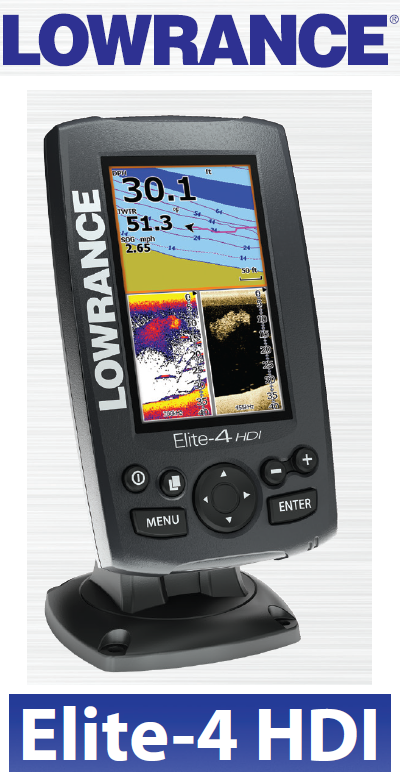
\includegraphics[width=6cm]{Vaje/KartGlobSlan/figs/ES.png}
	\caption{Globinomer proizvajalca \href{http://www.lowrance.com}{Lowrance}.}
	\label{fig:v_est_es}
\end{figure}

\noindent
Navodila za uporabo dobite na naslovu \href{https://drive.google.com/open?id=0B1dT-CBA07ANQU9sOU96MDJ5b2M}{link\_do\_vaje} v mapi \texttt{Lowrance\_Sonar/doc}, kjer si poglejte dokument \texttt{ELITE-4\_HDI\_User\_Guide.pdf}.

\noindent
Poleg uporabniškega priročnika imate tudi šifrant za NMEA stavke (\texttt{nmea\_output.pdf}), ki prihajajo iz naprave. V tem dokumentu imate opisane vse podatke, ki jih boste potrebovali pri obdelavi podatkov po opravljenih meritvah na morju.

\noindent
Sonar bo na barki potrebno pravilno namestiti in povezati z napajanjem, računalnikom in sondo. To boste storili v prisotnosti mentorja, ki vam bo v pomoč.

\subsubsection{Lowrance Monitor}
Lowrance Monitor je program s pomočjo katerega spremljamo osnovne podatke, ki prihajajo iz sonarja. Enako bo v pomoč pri shranjevanju podatkov iz sonarja na merilni točki. Vsako merilno točko (WP\_11, $\ldots$ , WP\_55, slika \ref{fig:v_est_wps}) bo potrebno z barko točno poiskati. Ko bomo na merilni točki pričnemo z meritvijo. Sprožimo snemanje podatkov iz sonarja in po potrebi zajamemo vzorec morja in spustimo Secchi-jev disk.

\begin{figure}[!h]
	\centering 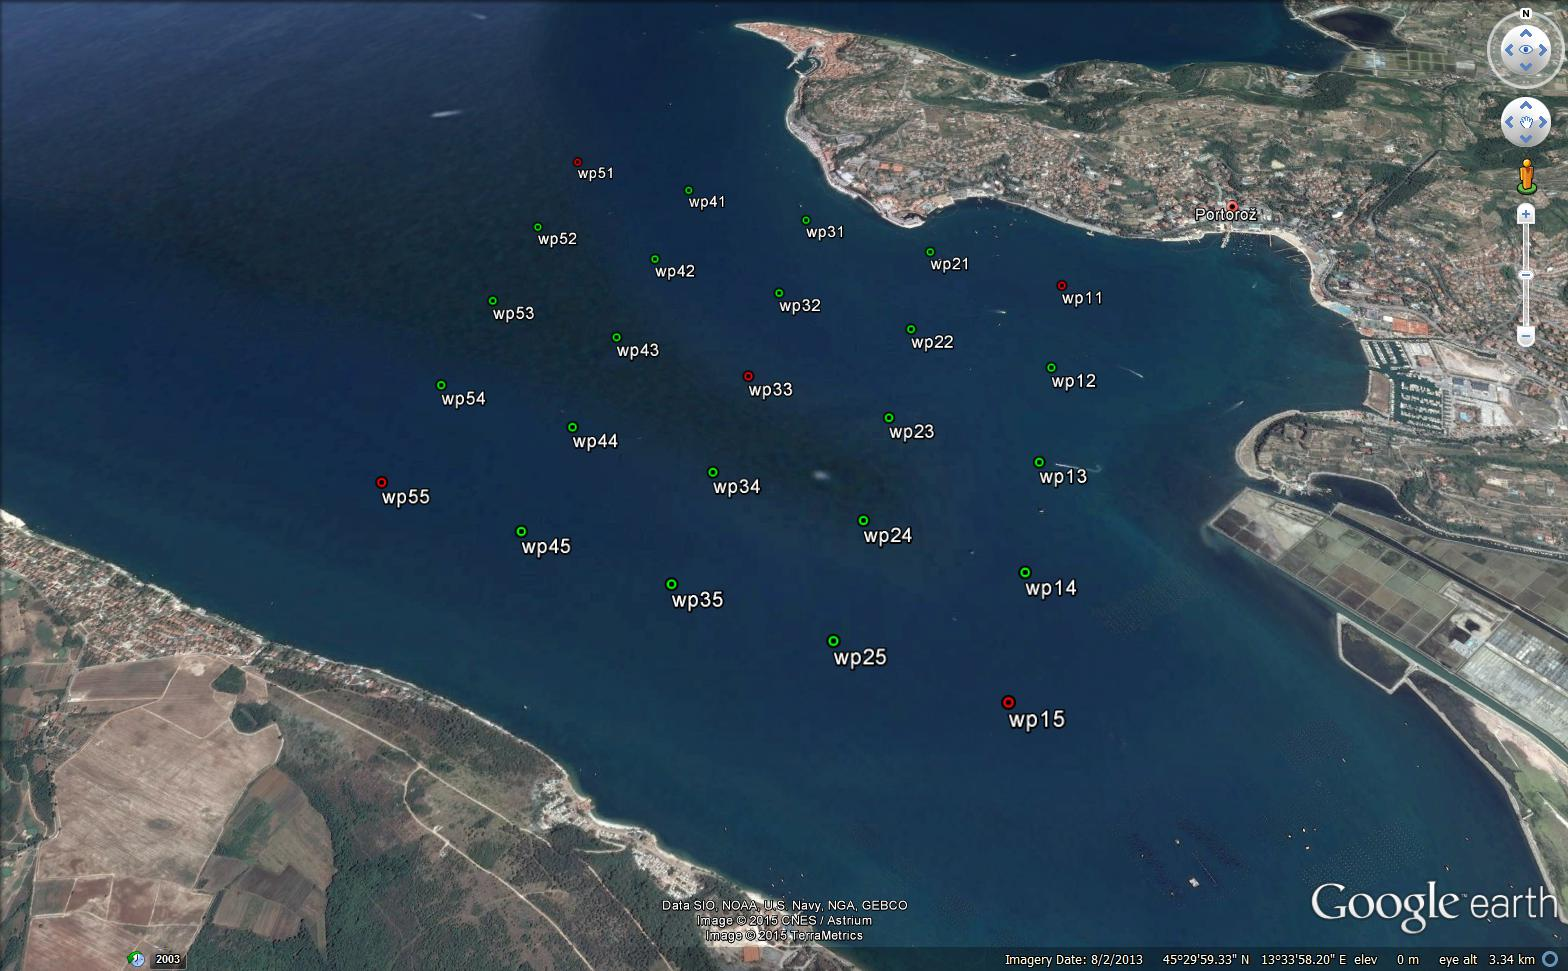
\includegraphics[width=12cm]{Vaje/KartGlobSlan/figs/track_01_02.jpg}
	\caption{Mreža merilnih točk (WP-WayPoint). Zelena točka pomeni meritev časa, položaja, globine in temperature, rdeča točka pomeni še dodatno meritev slanosti in prosojnosti. Točke so zapisane v datoteki \href{https://drive.google.com/open?id=0B1dT-CBA07ANWDI0dDdkc1p1TkU}{track\_01.kml}, je tekstovnega tipa in jo lahko pregledujete ali odprete z GoogleEarth.}
	\label{fig:v_est_wps}
\end{figure}

\newpage
\noindent
\textbf{Opis programa in postopek zagona:}
\vspace*{5mm}

\begin{figure}[!h]
	\begin{minipage}{5.5cm}
		\centering 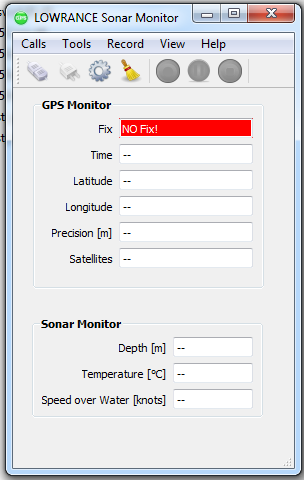
\includegraphics[width=5.5cm]{Vaje/KartGlobSlan/figs/no_fix.png}
	\end{minipage}
	\begin{minipage}{5.5cm}
		\centering 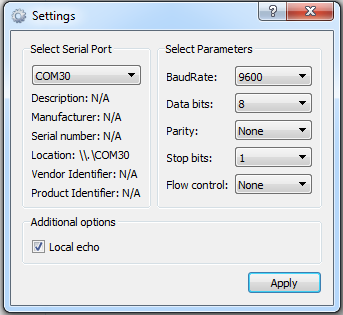
\includegraphics[width=5.5cm]{Vaje/KartGlobSlan/figs/connect.png}
		\vspace{3.3cm}
	\end{minipage}	
	\caption{Prikaz maske Lowrance Monitor programa (levo). Zgoraj imamo menu (Calls,...), pod imamo ToolBar z ikonami za upravljanje. Okno sestavljajo informacije iz GPS in Sonar naprave. Možnost je tudi spremljave podatkov direktno iz priklopa. Na desni sliki je prikaz okna za povezavo z napravo.}
	\label{fig:v_est_lmp_01}
\end{figure}

\begin{enumerate}
	\item \textbf{Nastavitev vhoda:}\\[1mm]
	Najprej pritisnemo gumb  
\includegraphics[width=5mm]{Vaje/KartGlobSlan/figs/icons/settings.png} (Settings), ki odpre okno Settings (desna slika na sliki \ref{fig:v_est_lmp_01}) in nastavimo Serial Port. Če je priklopljenih več naprav imamo možnost izbire različnih portov. S testiranjem izberemo pravilno (tista, ki prikaže vse podatke).\\[2mm]
	
	\item \textbf{Povezovanje naprave:}\\[1mm]
	Sedaj moramo napravo povezati. Pritisnemo gumb 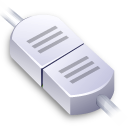
\includegraphics[width=5mm]{Vaje/KartGlobSlan/figs/icons/connect.png} (Connect), ki nas poveže z napravo. Če je vse vredu, se odpre dodatno okno, ki prikazuje tok surovih podatkov iz naprave. Hkrati se prične izpisovanje podatkov na monitorju GPSa in sonarja (slika \ref{fig:v_est_lmp_02}).\\[2mm]
	
	\begin{figure}[!h]
		\centering 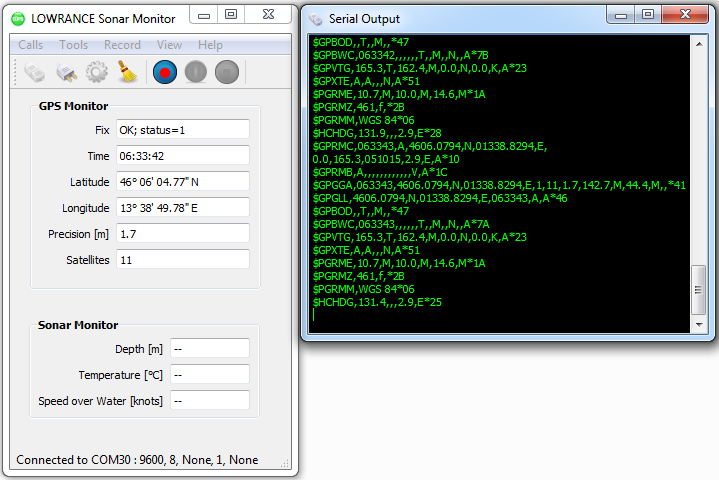
\includegraphics[width=10cm]{Vaje/KartGlobSlan/figs/connected.png}
		\caption{Prikaz povezane naprave in izpis podatkov na monitorju in konzoli.  Vidimo, da podati iz sonarja niso dostopni. Nekaj je narobe s sondo!}
		\label{fig:v_est_lmp_02}
	\end{figure}
	
	\item \textbf{Odklop vhoda:}\\[1mm]
	Lahko tudi preklapljamo med napravami. Napravo moramo najprej odklopiti iz  programa tako, da pritisnemo gumb 
\includegraphics[width=5mm]{Vaje/KartGlobSlan/figs/icons/disconnect.png} (Disconnect) in nato ponovimo postopek v točki 1. in 2.\\[2mm]
	
	\item \textbf{Snemanje podatkov:}\\[1mm]
	Ko smo prispeli na točko in je naprava povezana, bi radi pričeli s snemanjem podatkov. Pritisnemo gumb 
\includegraphics[width=5mm]{Vaje/KartGlobSlan/figs/icons/record.png} (Record) in pričnemo shranjevati podatke v spomin računalnika. Če ugotovimo, da smo se preveč odmaknili od točke in meritev še ni končana, lahko snemanje trenutno prekinemo s pritiskom na gumb 
\includegraphics[width=5mm]{Vaje/KartGlobSlan/figs/icons/pause.png} (Pause). Vsi posneti podatki so še vedno v spominu. Snemanje ponovno zaženemo z gumbom (Record). V primeru, da smo meritev zaključili, pritisnemo gumb 
\includegraphics[width=5mm]{Vaje/KartGlobSlan/figs/icons/stop.png} (Stop). Meritev je tako zaključena in jo lahko shranite v datoteko. Recimo ste na točki WP\_11 in podatke shranite v datoteko z imenom \texttt{wp\_11.nmea} (slika \ref{fig:v_est_lmp_03}). Ko podatke shranimo se izbrišejo iz spomina in je program pripravljen za ponovno snemanje od začetka.\\[2mm]
	
	\begin{figure}[!h]
		\centering 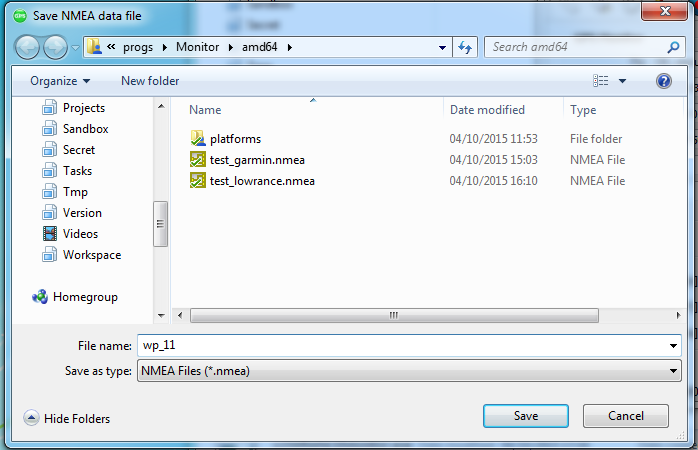
\includegraphics[width=8cm]{Vaje/KartGlobSlan/figs/save.png}
		\caption{Prikaz shranitve podatkov v datoteko.}
		\label{fig:v_est_lmp_03}
	\end{figure}
	
\end{enumerate}


\subsection{Prosojnost}
Meritve prosojnosti s pomočjo Secchi diska (bela okrogla plošča premera 30cm) so enostavne, le na začetku je potrebna umeritev Secchi-jeve globine za naš zaliv. Kako poteka umeritev si lahko preberete v članku \href{https://drive.google.com/open?id=0B1dT-CBA07ANSFBneFpLSXV1SjQ}{Secchi\_Universality} in \href{https://drive.google.com/open?id=0B1dT-CBA07ANbmRIQkZieUhGYVE}{doktoratu}.\\[5mm]

\noindent
Meritev je preprosta. Secchijev disk spustimo v morje. Spuščamo ga toliko časa, da nam izgine. Izmerimo na kateri globini je izginil in ga potegnemo ven. S pomočjo umeritvenih tabel določimo indeks prosojnosti $k$.

\noindent
Ena od metod je tudi določitev iz grobe funkcije:
\begin{equation}
\label{eq:v_est_secchi}
k(Z_D) = \frac{\alpha}{Z_D^{\beta}},
\end{equation}

\begin{minipage}{4cm}
	\noindent
	kjer sta konstanti
	
	\begin{align*}
	\alpha & = 1.64192243,\\
	\beta  & = 0.963815813.
	\end{align*}
	
	\noindent
	Graf funkcije (\ref{eq:v_est_secchi}) je prikazan na sliki desno.
\end{minipage}
\begin{minipage}{7.5cm}
	\centering 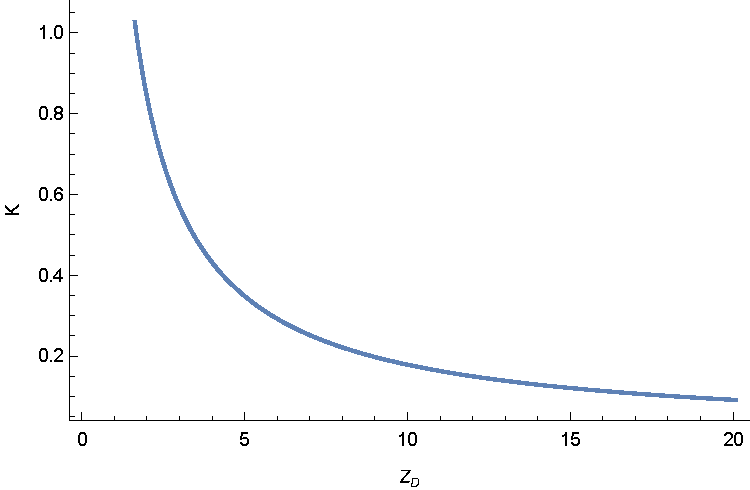
\includegraphics[width=7cm]{Vaje/KartGlobSlan/figs/secchi_func.pdf}
\end{minipage}

\newpage
\section{Naloga}
Študentje morajo izmeriti različne fizikalne parametre na prej zadanih točkah na morju (WP - WayPoint), kot je prikazano na sliki \ref{fig:v_est_wps}. Točna lokacija točk je zapisana v \href{https://drive.google.com/open?id=0B1dT-CBA07ANWDI0dDdkc1p1TkU}{\texttt{track\_01.kml}} datoteki.\\[5mm]

\noindent
V vseh točkah snemamo odčitke iz sonarja 60 sekund. Sonar posname čas, položaj, globino in temperaturo. Dodatno je potrebno na točkah, ki so obarvane rdeče \texttt{wp\_11}, \texttt{wp\_15}, \texttt{wp\_51}, \texttt{wp\_55} in \texttt{wp\_33} izmeriti tudi slanost in indeks prosojnosti.\\[5mm]

\noindent
Po opravljenih meritvah je potrebno podatke iz sonarja obdelati.
\begin{itemize}
	\item iz meritev za vsako točko je potrebno določiti povprečni položaj, globino in temperaturo,
	\item potrebno je izrisati 3D graf globin, ki prikazujejo povprečen izmerjen relief,
	\item izdelati tabelo z rezultati,
	\item napisati poročilo (rezultati, analiza in zaključek).
\end{itemize}

\noindent
Za obdelavo podatkov uporabite \textsc{MatLab} okolje. Na \href{https://drive.google.com/open?id=0B1dT-CBA07ANSXl2YmIxcXdUQkk}{lokaciji} je program za branje NMEA podatkov iz nmea datoteke. Nakazana je tudi smiselna uporaba za analizo.

